\subsubsection*{4.a}
On donne le droit de créer des tables et utilisateurs a admin depuis DBAIOT

\lstinputlisting[style=sqlstyle]{SQL/Partie4/grant1.sql}

\begin{center}
    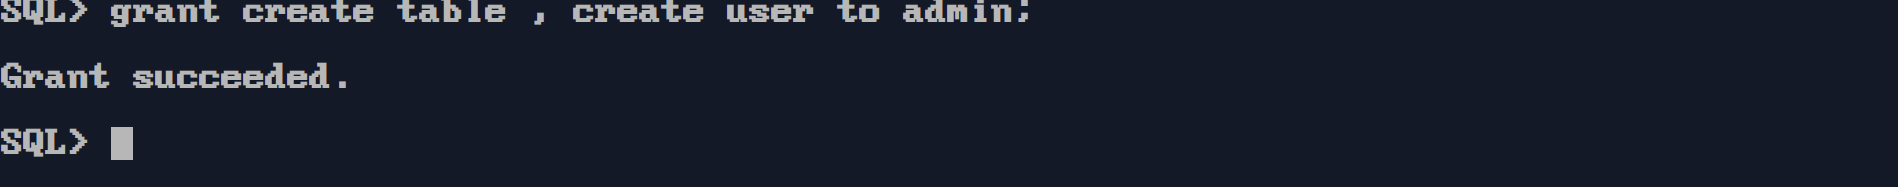
\includegraphics[width=\textwidth]{ScreenShot/Partie4/grant1.png}
\end{center}

\subsubsection*{4.b}
Pour verifie les droit de admin on va afficher la table USER\_SYS\_PRIVS 

\lstinputlisting[style=sqlstyle]{SQL/Partie4/verify1.sql}

\begin{center}
    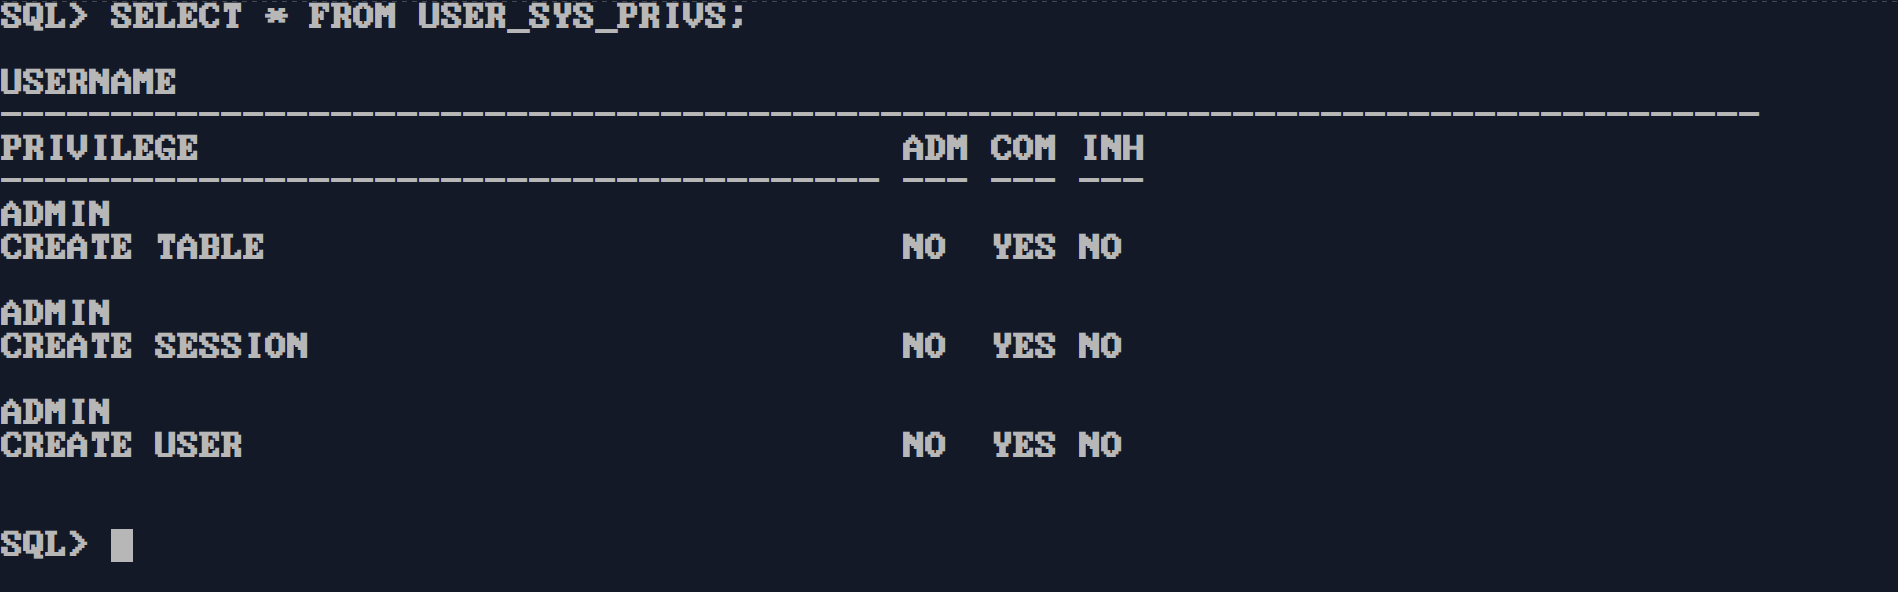
\includegraphics[width=\textwidth]{ScreenShot/Partie4/verify1.png}
\end{center}

\begin{prettyBox}{Remarque}{myblue}
La table USER\_SYS\_PRIVS affiche les privilèges du user avec lequel on
est connecté. La colonne ADM (admin) indique que l'utilisateur peut accorder 
ou révoquer ce privilège, COM (command) signifie que l'utilisateur a droit
à ce privilège, et INH (inherit) indique que l'utilisateur a obtenu ce privilège 
indirectement via un role.
\end{prettyBox}

